\chapter{Introduction}

Neutrinos have been at the forefront of discovery since their prediction by W. Pauli, who proposed in 1930 the existence of a neutral, unobserved particle to explain the apparent violation of energy conservation in beta decay \cite{betaspectrum}. He admitted that neutrinos (then deemed ``neutrons'' -- what we now know as neutrons had not been discovered yet either) should be difficult to observe experimentally, but also that it seemed unlikely that they would never have been noticed before.  As it turns out, they are much more difficult to observe than he predicted; they will not be noticed without extreme experimental techniques.

A theory formulated in 1933 by E. Fermi for beta decay \cite{FermiBetaDecay}, including the neutrino, would be the beginnings of weak theory, and the development of the very successful Standard Model (SM) of particle physics.  However, the SM assumes that neutrinos are massless.  The discovery of non-zero neutrino mass via neutrino oscillations in the late 1990s \cite{SuperK} shows that there is more new physics to be discovered -- a path to follow in the further unification of physical theory.

Neutrinos are extremely difficult to study, but the rewards are profound.  The favored See-saw Mechanism is a theory which predicts the extreme lightness of neutrinos, while also predicting very heavy neutrinos.  The existence of heavy neutrinos in the high-energy environment of the early universe, coupled with the possibility of the violation of CP conservation which could slightly favor the production of matter vs. anti-matter in decays of these heavy neutrinos, could explain why the universe exists as we know it.  
\cite{SeeSaw}

If this theory is correct, then neutrinos would be described by the Majorana formulation rather than Dirac, and the process of neutrinoless double beta decay ($0\nu\beta\beta$) would be allowed.  Observation of $0\nu\beta\beta$ would simultaneously demonstrate that neutrinos are Majorana particles, as well as give a measurement of the absolute mass itself \cite{effectiveMass}.  This chapter outlines the current theory for neutrinos, and then describes the $0\nu\beta\beta$ experiments EXO-200 and nEXO, in order to motivate barium tagging for nEXO.

\section{Neutrinos}

Neutrinos are chargeless leptons which only interact via the weak force (and gravity).  There are three known ``flavors'' of neutrinos, each corresponding to one of the three known leptons:  $\nu_{e}$, $\nu_{\mu}$, and $\nu_{\tau}$.  These are the eigenstates in the basis of the weak force, so they are the states in which a neutrino will interact via the weak force.

\subsection{Neutrino Oscillation and Mass}

The postulate that neutrinos have an energy basis which is different from the flavor basis predicts the phenomenon of oscillation -- that the time evolution of an initially pure flavor state (as a neutrino will be produced) will result in a time-dependent probability of measuring the other two flavors as well.  

The very small mass of a neutrino (assumed zero in the SM), specifically relative to its momentum, lets one write its Hamiltonian in terms of mass squared differences $\Delta m_{ij}^{2} = m_{i}^{2} - m_{j}^{2}$, where $i$,$j$ = 1,2,3, referring to what we then call mass states.  The mass basis is really the energy basis with the small mass approximation, along with dropping some constant terms in the Hamiltonian (which do not affect time evolution).  Writing the time evolution in terms of mass squared differences means that neutrino oscillation experiments can produce measurements of these differences.  In fact, the discovery of neutrino oscillation was the first (and only, so far) demonstration that neutrinos have a non-zero mass.  Without neutrino mass (particularly without differences between the masses of the mass states), neutrinos would not oscillate.

Neutrino oscillation experiments also provide measurements on the amount of mixing between the flavor basis and the mass basis.  We define the mixing between them by a rotation in terms of three mixing angles, $\theta_{12}$, $\theta_{23}$, and $\theta_{13}$.  Transformation between the flavor and mass bases is done with the following unitary matrix, called the Pontecorvo--Maki-–Nakagawa–-Sakata (PMNS) matrix:

\begin{equation}
\begin{aligned}
U &= \begin{pmatrix}
1 & 0 & 0 \\
0 & c_{23} & s_{23} \\
0 & -s_{23} & c_{23} \end{pmatrix}
\begin{pmatrix}
c_{13} & 0 & s_{13} e^{-i \delta} \\
0 & 1 & 0 \\
-s_{13} e^{i \delta} & 0 & c_{13} \end{pmatrix}
\begin{pmatrix}
c_{12} & s_{12} & 0 \\
-s_{12} & c_{12} & 0 \\
0 & 0 & 1 \end{pmatrix}
\begin{pmatrix}
1 & 0 & 0 \\
0 & e^{i \alpha_{1}/2} & 0 \\
0 & 0 & e^{i \alpha_{2}/2} \end{pmatrix} \\
& = \begin{pmatrix}
c_{12} c_{13} & s_{12} c_{13} & s_{13} e^{-i \delta} \\
-s_{12} c_{23} - c_{12} s_{23} s_{13} e^{i \delta} & c_{12} c_{23} - s_{12} s_{23} s_{13} e^{i \delta} & s_{23} c_{13} \\
s_{12} s_{23} - c_{12} c_{23} s_{13} e^{i \delta} & -c_{12} s_{23} - s_{12} c_{23} s_{13} e^{i \delta} & c_{23} c_{13} \end{pmatrix}
\begin{pmatrix}
1 & 0 & 0 \\
0 & e^{i \alpha_{1}/2} & 0 \\
0 & 0 & e^{i \alpha_{2}/2} \end{pmatrix}
\end{aligned}
\label{eqn:umatrix}
\end{equation}

\noindent
where $c_{ij} = \cos \theta_{ij}$ and $s_{ij} = \sin \theta_{ij}$.  $\delta$ is a phase factor related to lepton CP violation, and $\alpha_{i}$ are Majorana phases.

Studying oscillations of neutrinos from different kinds of sources, with different energies and path lengths, can isolate sensitivities to the different parameters.  For example, the study of solar neutrinos (neutrinos emanating from nuclear fusion reactions in the core of the sun) provides sensitivity to $\theta_{12}$ and $\Delta m_{12}^{2}$.  The oscillation parameters so far measured shown in Table  \ref{table:nu_osc_vals}:

\begin{table}[!htbp]
\caption{Best-fit values for neutrino oscillation parameters, from a global fit to oscillation experiment data.   Parameters which depend on the mass hierarchy have values for NH (IH).  The atmospheric parameter $\Delta m^{2}$ is defined as $\Delta m^{2} = \Delta m^{2} = \Delta m_{31}^{2} - \Delta m_{21}^{2}/2 > 0 (\Delta m^{2} = \Delta m_{32}^{2} + \Delta m_{21}^{2}/2 < 0)$. \cite{ReviewNuMass}} %not sure what [Small Table], between \caption and {}, w/ no spaces, does
\label{table:nu_osc_vals}
\begin{tabular}{c|c}
Parameter & Measurement ($\pm 1 \sigma$) \\
\hline
$\Delta m_{12}^{2}$ & 7.54$^{+0.26}_{-0.22}$ 10\textsuperscript{-5}~eV\textsuperscript{2}\\
$|\Delta m^{2}|$ & 2.43 $\pm$ 0.06 (2.38 $\pm$ 0.06) 10\textsuperscript{-3}~eV\textsuperscript{2}\\
$\sin^{2} \theta_{12}$ & 0.308 $\pm$ 0.017\\
$\sin^{2} \theta_{23}$ & 4.37$^{+0.033}_{-0.023}$ (4.55$^{+0.039}_{-0.031}$)\\
$\sin^{2} \theta_{13}$ & 0.0234$^{+0.0020}_{-0.0019}$ (0.0240$^{+0.0019}_{-0.0022}$)\\
$\delta / \pi$ (2$\sigma$ range)& 1.39$^{+0.38}_{-0.27}$ (1.31$^{+0.29}_{-0.33}$)\\
\end{tabular}
\end{table}

Note that only the absolute value of the atmospheric neutrino oscillation parameter $\Delta m^{2}$ is known.  As a consequence, there are two possibilities for the hierarchy of the three neutrino masses.  These are called the Normal and Inverted Hierarchies, as shown in Fig. \ref{fig:numasshier}.

\begin{figure}[H]
        \centering
                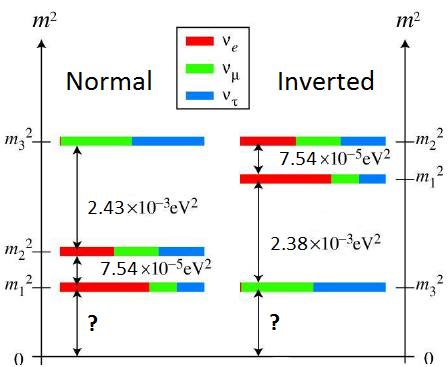
\includegraphics[width=.5\textwidth]{figures/hierarchy_alterred.png}
                \caption{The two possible hierarchies of neutrino masses.  The colors depict the mixing between the mass and flavor bases.}
\label{fig:numasshier}
\end{figure}

\noindent
The correct mass hierarchy remains unknown, but next-generation neutrino experiments, possibly including nEXO, will be able to discern this.

Neutrino oscillation demonstrates that neutrinos have non-zero mass, and though oscillation experiments measure the mass squared differences, we still do not have a measurement of the absolute masses of the three neutrinos.  Cosmology can put limits on the sum of the three neutrino masses.  The Planck collaboration reports an upper bound on this sum at $\sum\limits_{i} m_{i} < 0.23$~eV \cite{Planck}.  The KATRIN experiment will search for absolute neutrino mass with limiting capability of $m_{\bar{\nu}_{e}} < 0.2$~eV (90\% CL) by measuring the spectrum of tritium beta decay near the Q-value, searching for deviation from the spectrum with zero neutrino mass \cite{KATRIN}.

\section{Double Beta Decay}

Double beta decay is the simultaneous decay of two neutrons in a nucleus into two protons and two electrons.  Two-neutrino double beta decay ($2\nu\beta\beta$), shown in Fig. \ref{fig:feynman_diags}(left), is allowed by the Standard Model and has been observed in eleven isotopes with half-lives between $10^{19}$ and $10^{21}$ years.  Similar to beta decay, a neutrino accompanies each electron in this decay, broadening the spectrum of the summed electron energy. This is a second-order process, making it a rare decay, and requiring low backgrounds to measure.

\begin{figure}[H]
        %\centering
        %\begin{subfigure}
                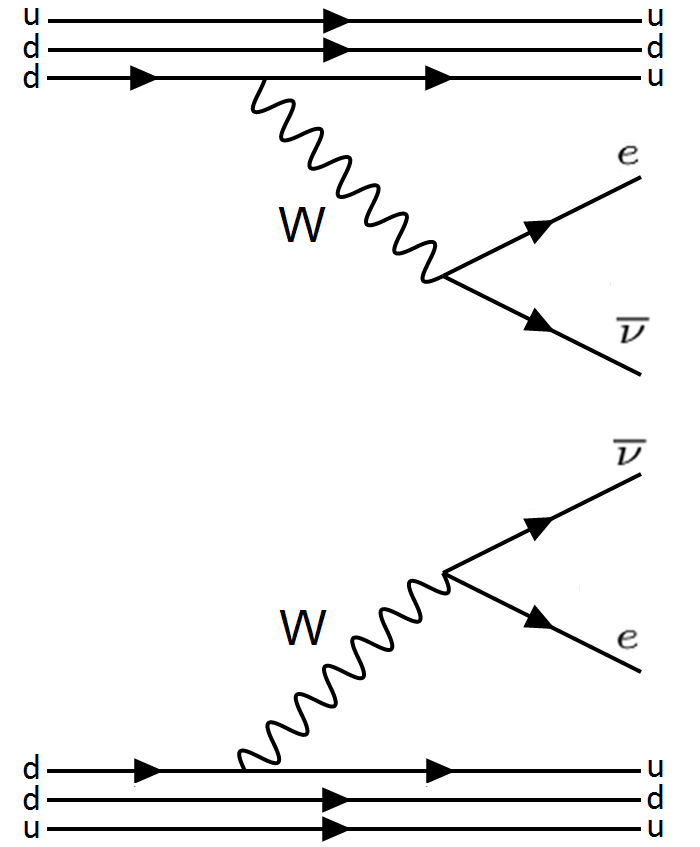
\includegraphics[width=.35\textwidth]{figures/feynman_2nu_quarks.png}
                %\caption{barf}
%        %\end{subfigure}
        %\begin{subfigure}
                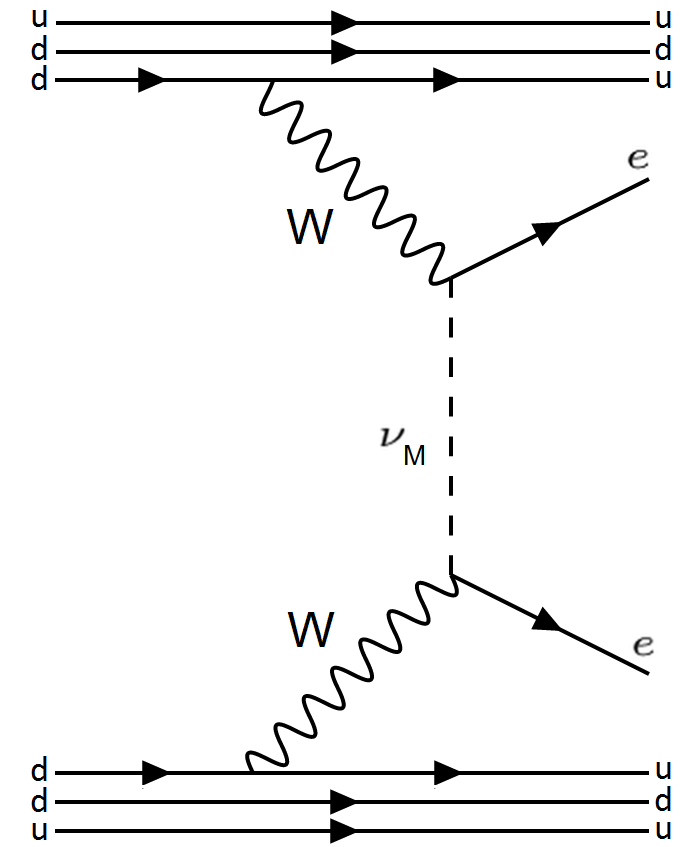
\includegraphics[width=.35\textwidth]{figures/feynman_0nu_quarks.png}
                \caption{Two-neutrino (left) and neutrinoless (right) double beta decay.}
        %\end{subfigure}
        \label{fig:feynman_diags}
\end{figure}

%\begin{table}[!htbp]
%\caption{$2\nu\beta\beta$ half-lives measured for various isotopes.} %not sure what [Small Table], between \caption and {}, w/ no spaces, does
%\label{table:bb_isotopes}
%\begin{tabular}{c|c|c}
%Isostope & $T^{2\nu}_{1/2} (10^{21}$~y) & Experiment\\
%\hline
%$^{136}$Xe & $2.165 \pm 0.016 \pm 0.059$ & EXO-200\\
%$^{76}$Ge & $1.84^{+0.14}_{-0.10}$ & GERDA\\
%\end{tabular}
%\end{table}

$0\nu\beta\beta$, shown in Fig. \ref{fig:feynman_diags}(right), is a postulated mode of double beta decay. In this case, the neutrino is exchanged as a virtual particle (which would require that it is a Majorana particle), and there are no neutrinos in the final products. If discovered, not only would neutrinos be determined Majorana particles, but their absolute mass could also be measured as it relates to the $0\nu\beta\beta$ half-life according to Eqn. \ref{eqn:rate_vs_mass}:

\begin{equation}
T_{1/2}^{0\nu} = (G^{0\nu}(Q,Z)|M^{0\nu}|^{2}\braket{m_{\nu}}^{2})^{-1}
\label{eqn:rate_vs_mass}
\end{equation}

\noindent
where $T_{1/2}^{0\nu}$ is the $0\nu\beta\beta$ half-life,  $G^{0\nu}$ is a known phase space factor, and $M^{0\nu}$ is a model-dependent nuclear matrix element. The effective electron neutrino mass $\braket{m_{\nu}}$ is the expectation value of the mass for a pure electron neutrino:

\begin{equation}
\braket{m_{\nu}} = \sum\limits_{i} U_{ei}^{2} m_{i}.
\label{eqn:effectivemass}
\end{equation}

The sum of the energies of the emitted electrons in double beta decay will serve as the distinction between the two-neutrino and zero-neutrino modes, shown in Fig. \ref{fig:spectrum_bb}. In the two-neutrino mode, the total decay energy is shared probabilistically between the electrons and the neutrinos (the nucleus recoil energy is negligible), resulting in a broad distribution in the summed electron energy. (Recall the similarly broad electron energy in single beta decay, which ultimately led to discovery of the neutrino involved.) But in the zero-neutrino mode, all of the decay energy is carried away by the two electrons, resulting in only a single allowed value for the summed electron energy -- a peak in the summed electron energy spectrum at the Q-value. 

\begin{figure}[H]
        \centering
                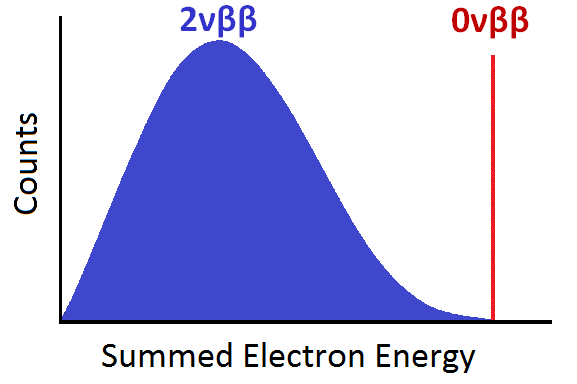
\includegraphics[width=.7\textwidth]{figures/spectrum_bb.png}
                \caption{Conceptual two-neutrino (blue) and zero-neutrino (red) double beta decay spectra.}
\label{fig:spectrum_bb}
\end{figure}

The rarity of double beta decay requires very low backgrounds, especially around the Q-value for the $0\nu\beta\beta$ search. The next sections describe the experiments EXO-200 and it's next-generation successor, nEXO.

\section{Enriched Xenon Observatory}

EXO-200 and nEXO (EXO standing for Enriched Xenon Observatory) are a progression of two experiments, each a LXe time projection chamber (TPC) designed to study the double beta decay of the isotope \textsuperscript{136}Xe, and ultimately to search for the zero-neutrino mode.  Xe is fairly unique among the double beta decay isotopes in that it can be studied in a gas or liquid TPC instead of solid crystals or foils.  The 3D event position reconstruction abilities of a TPC have advantages in background reduction, described in section \ref{subsec:EXO200}.  Purification of Xe is straightforward and can be done continuously in a detector.  LXe is transparent, and produces substantial ionization and scintillation at 178~nm when energy is deposited in the LXe \cite{EXO200TwoNuLong}.  Also, the ratio between observed scintillation light and remaining ionized electrons (drifted from the decay site by the TPC's electric field) exhibits a well-known microscopic anti-correlation \cite{anticorr}, the understanding of which improves the energy resolution of the detector.  Finally, a liquid TPC approach offers the opportunity to identify, or ``tag'', the daughter Ba\textsuperscript{++} at the site of the double beta decay event, which would provide a background-free identification of $0\nu\beta\beta$ \cite{Moe1991}. Barium tagging is the focus of our group at CSU and is the subject of this thesis.

The following sections decribe the EXO-200 experiment, as well as nEXO, the next-generation tonne-scale LXe TPC which is now in the design stages.  EXO-200 does not have barium tagging implemented, but it is hoped that nEXO will. 

\subsection{EXO-200}
\label{subsec:EXO200}

EXO-200 has been operational since 2011.  It is a TPC using 110~kg of active LXe enriched to 80.672\% $\pm$ 0.14\% \textsuperscript{136}Xe \cite{EXO200TwoNuLong},  designed to probe Majorana neutrino masses down to around 109-135~meV (the range covers different matrix element calculations) \cite{EXO200instrumentationPart1}, and is located about half a mile underground in the Waste Isolation Pilot Plant (WIPP) near Carlsbad, NM.  This mine is in a salt basin, which contains lower levels of Uranium and Thorium than a more typical mine in rock.

A schematic of the TPC in the class 100 cleanroom is shown in Fig. \ref{fig:cleanroom}.  Several layers of lead wall surround the copper cryostat, which is filled with HFE-7000, a cryogenic fluid which keeps the TPC cooled to LXe temperatures, as well as aids in shielding.  The TPC vessel is made of low-radioactivity copper, and is kept as thin as possible to minimize backgrounds.  Scintillating panels on the outside of the cleanroom provide muon veto.

\begin{figure}[H]
	\centering
	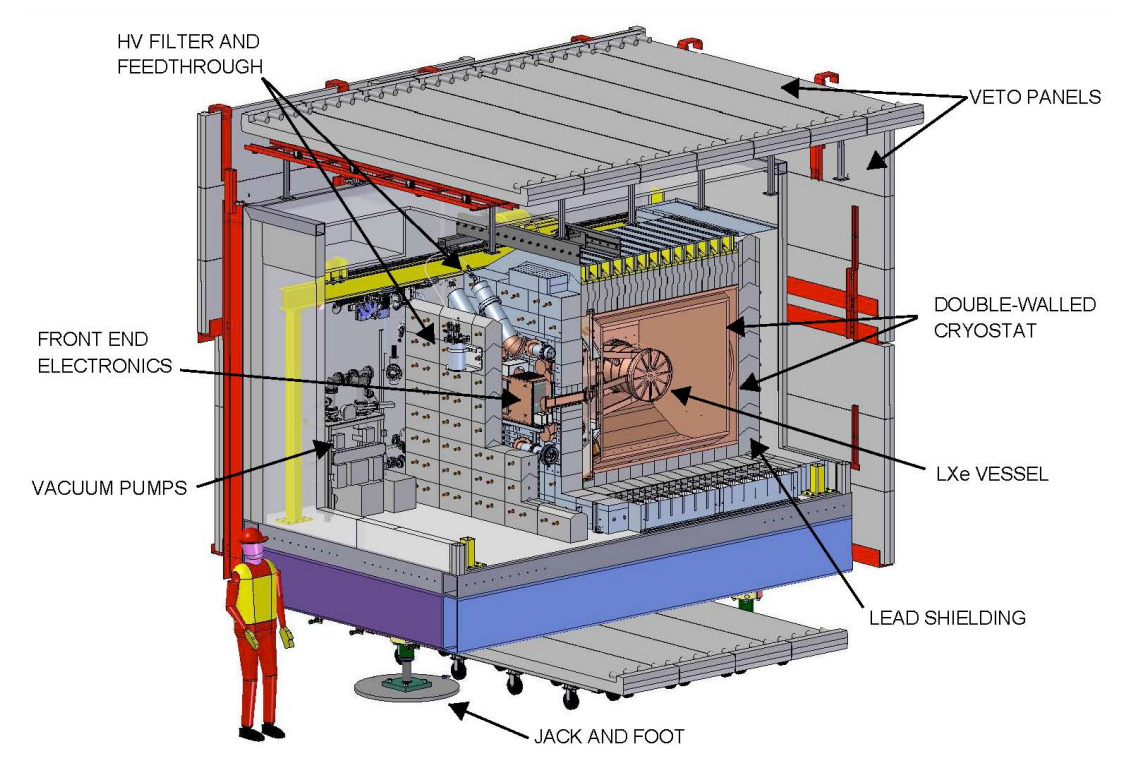
\includegraphics[width=.7\textwidth]{figures/cleanroom.png}
	\caption{Drawing of cleanroom laboratory in the WIPP drift.}
\label{fig:cleanroom}
\end{figure}

A cut-away view of the EXO-200 detector is shown in Fig. \ref{fig:tpc}.  It is two mirrored TPCs which share a cathode.  The detection planes are a combination of ionized charge induction/collection wires and large area avalanche photodiodes (LAAPDs) which detect scintillation light \cite{APDs}.

\begin{figure}[H]
	\centering
	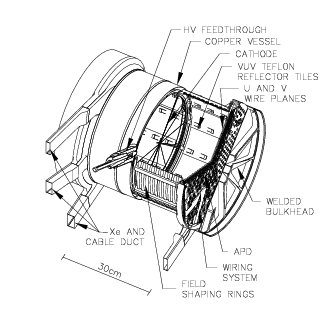
\includegraphics[width=.9\textwidth]{figures/TPC.png}
	\caption{EXO-200 TPC cutaway \cite{EXO200TwoNuLong}.}
\label{fig:tpc}
\end{figure}

A photograph of the detection plane is shown in Fig. \ref{fig:tpcphoto}, and a schematic of event detection is shown in Fig. \ref{fig:detectionplane}.  When a double beta decay event occurs in the LXe, the energetic electrons ionize many surrounding Xe atoms.  Some electrons very quickly recombine, emitting scintillation light which is collected by the LAAPDs.  This is part of the energy collection, and also provides a time stamp for the event.  

\begin{figure}[H]
	\centering
	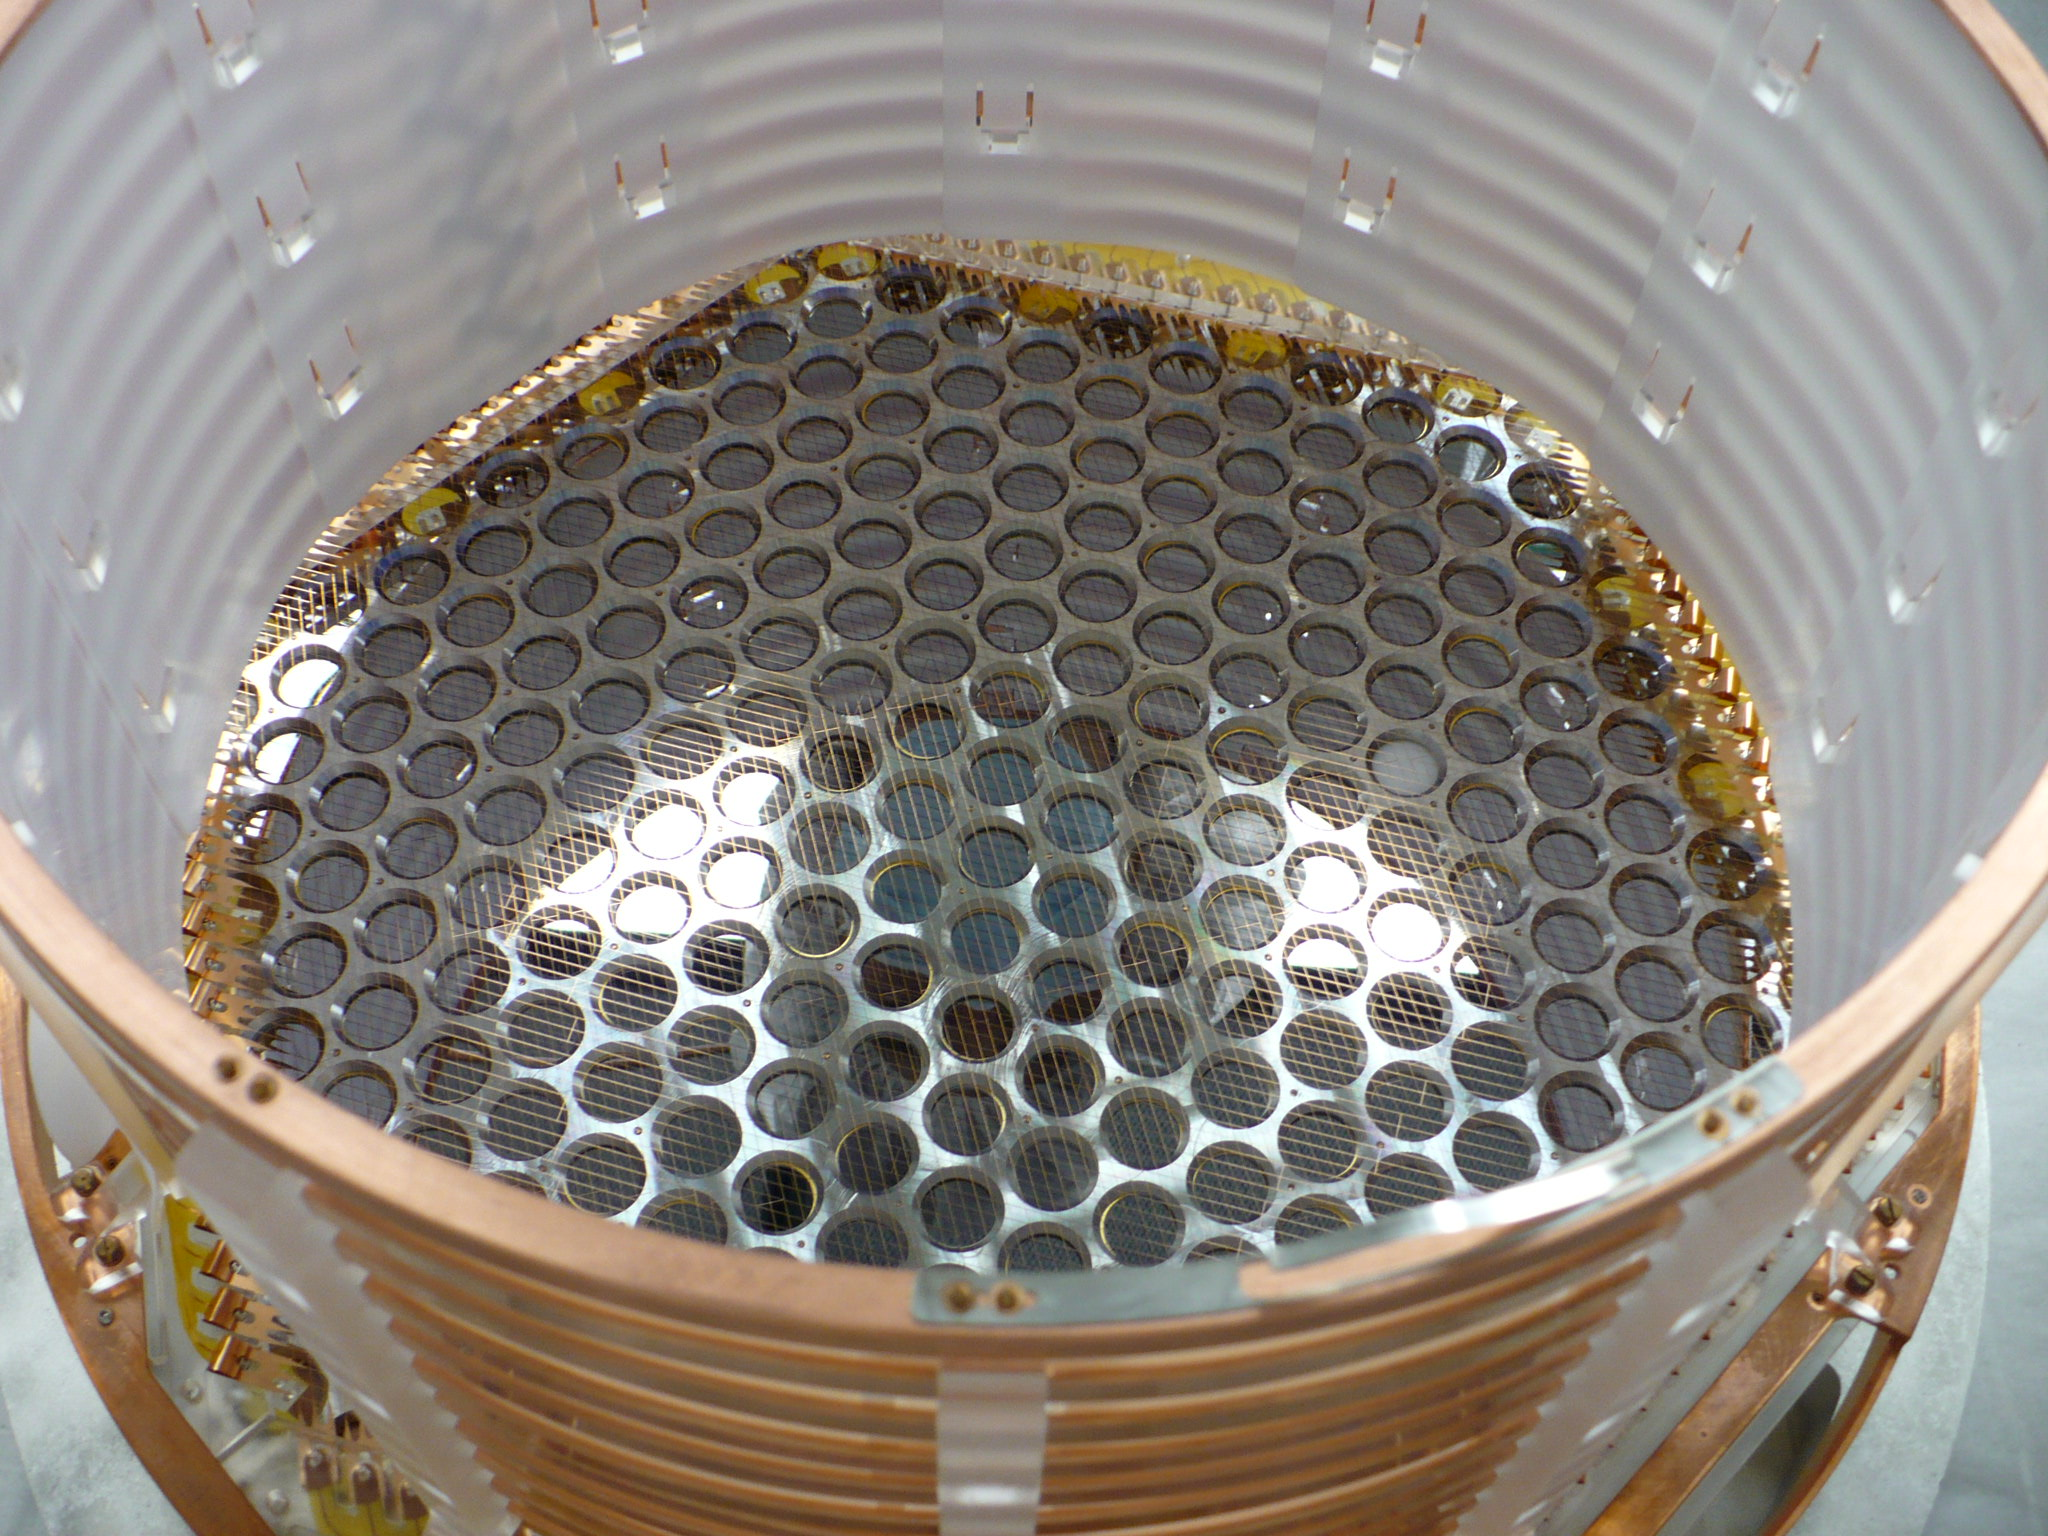
\includegraphics[width=.9\textwidth]{figures/TPCphoto.jpeg}
	\caption{View of the detection plane in one of the two EXO-200 TPCs.}
\label{fig:tpcphoto}
\end{figure}

The cathode is set to -8~kV, providing an electric field of 374~V/cm across the 20~cm drift length of each TPC.  Ionized electrons drift from the decay site, first passing the v-wires, which receive an induction signal, and are then collected by the u-wires, which are set at a 60$^\circ$ angle from the v-wires.  An electric field of 778~V/cm between the u- and v-wires ensures 100\% v-wire transparency.  The charge collection provides the remainder of the energy collection of the initial decay.  Together, the u- and v-wires give an x/y position measurement for the event.  The time between the initial scintillation detection and the charge collection give a z position, and a 3D position can be reconstructed for the event.  \cite{EXO200TwoNuLong}

\begin{figure}[H]
	\centering
	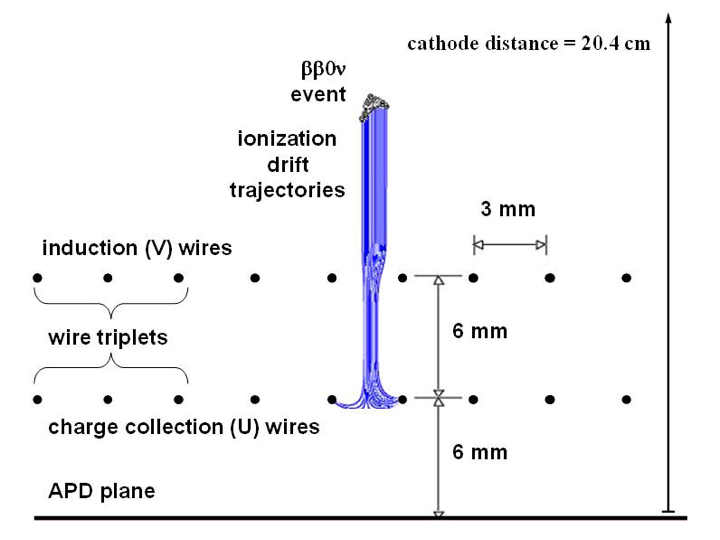
\includegraphics[width=.7\textwidth]{figures/anodecathodedriftcharges.png}
	\caption{EXO-200 event detection.  }
\label{fig:detectionplane}
\end{figure}

Having a reconstructed 3D event position is important in several ways.  Firstly, position-based corrections on scintillation and charge collection can be applied.  For charge, electronegative impurities in the LXe will absorb the drifting charge, requiring a drift-length (z-position) correction.  High purity levels, measured in terms of electron lifetime, of 2-3$\times 10^{3}~\mu$s are maintained in EXO-200, resulting in a small correction of few \% for maximal drift lengths.  For scintillation, a full 3D correction is applied (called the Light Map), as some regions have more efficient light collection by the LAAPDs [ref, maybe for whole paragraph].  A 3D position also allows a fiducial volume to be defined.  The effect of radioimpurities on detector surface, e.g. radon daughters collecting on the cathode, is mitigated by defining a stand-off distance required for events used in analysis.  \cite{EXO200TwoNuLong}

\textbf{\color{red}here:  }Finally, 3D reconstruction allows the distinction between single-site (SS) and multi-site (MS) events.  A(n?) MS event is one where two spatially separated events occur in the same [???]-$\mu s$ time window.  These are mostly caused by gamma rays interacting in the LXe, which can Compton-scatter several times.  Rejecting MS events strongly separates gamma events from double beta decay events.

Of course, barium tagging will also require a 3D reconstructed position in nEXO.

Calibration of EXO-200 is done using various radioactive sources which can be moved to several positions around the outside of the TPC.  Several different sources span the energy range of interest, but the main source is $^{228}$Th, which produces gamma rays at [???]~MeV, near the Q-value of $^{136}$Xe double beta decay where the $0\nu\beta\beta$ peak will be.  Source calibration data also provides a comparison between data and Monet-Carlo simulation, and provides the data for purity measurement and Light Map determination.  Data and Monte-Carlo for $^{228}$Th are shown in Fig. [ref fig source agreement].

The relationship between scintillation and ionization for a given event in LXe exhibits a well-known anti-correlation.  Applying this to the combination of those signals improves the energy resolution, shown in Fig. [ref fig anticorrelation].  This correction defines a combined energy axis, called the rotated energy.  Energy resolution is important in a $0\nu\beta\beta$ search, as it distinguished those events from $2\nu\beta\beta$ events in the tail of their spectrum.  Resolution of [???] is achieved in [ref $0\nu$ paper].

The final data set is fit using a combination of probability distribution functions (PDFs) for $0\nu\beta\beta$, $2\nu\beta\beta$, and all possible backgrounds.  Fig. \ref{fig:exo200data} shows the fits to the final energy spectrum data for (a) SS events, and (b) MS events.  The green bands beneath each plot show the residuals vs. energy.  The $2\nu\beta\beta$ spectrum, in gray, dominates the backgrounds in the SS spectrum.  The red dotted lines in the SS spectrum outline the {\color{red}2} $\sigma$ region of interest around the Q-value, where the $0\nu\beta\beta$ peak will lie.  The insets are a zoom into this region.  The fit value for $0\nu\beta\beta$ in this dataset is non-zero, but it is not statistically significant enough to claim discovery [ref nature].

\begin{figure}[H]
	\centering
	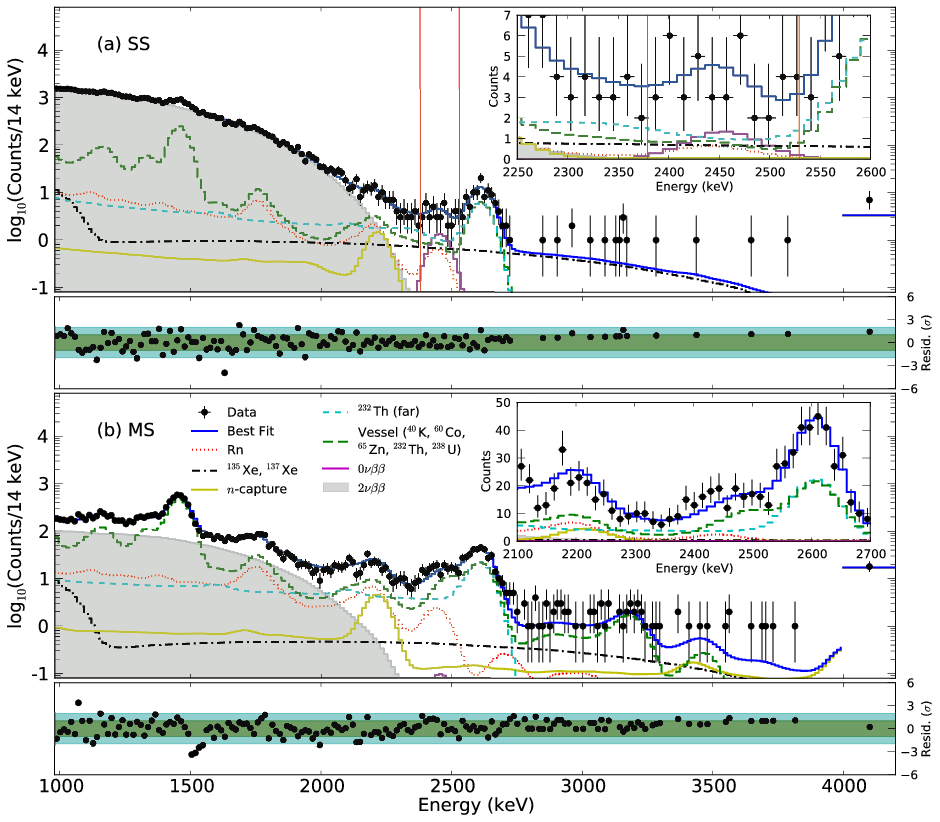
\includegraphics[width=.7\textwidth]{figures/exo_200_results.png}
	\caption{EXO-200 energy spectrum.  }
\label{fig:exo200data}
\end{figure}

[ref nature] reports the most accurate measurement of the $2\nu\beta\beta$ of $^{136}$Xe to date, at [???], and reports a limit on the half-life of $0\nu\beta\beta$ of $^{136}$Xe of [???] at the {\color{red}95~\%} confidence level, which translates to an upper limit on the Majorana neutrino mass between [???] and [???], depending on the method of calculation for [which param?].

\subsection{nEXO}

The next-generation successor to EXO-200 is nEXO, a tonne-scale LXe TPC which will probe Majorana neutrino masses down to the [???] scale [ref].  The sensitivity projections for nEXO are shown in Fig. \ref{fig:sensitivity_nEXO}, along with those of EXO-200.  nEXO will reach phase space where the two possible mass hierarchies begin to split; if nEXO successfully observes $0\nu\beta\beta$ in these regions, it may be able to also determine the mass hierarchy.  Barium tagging will push the sensitivity further into the region allowed only by the normal hierarchy [ref for this?].

\begin{figure}[H]
	\centering
	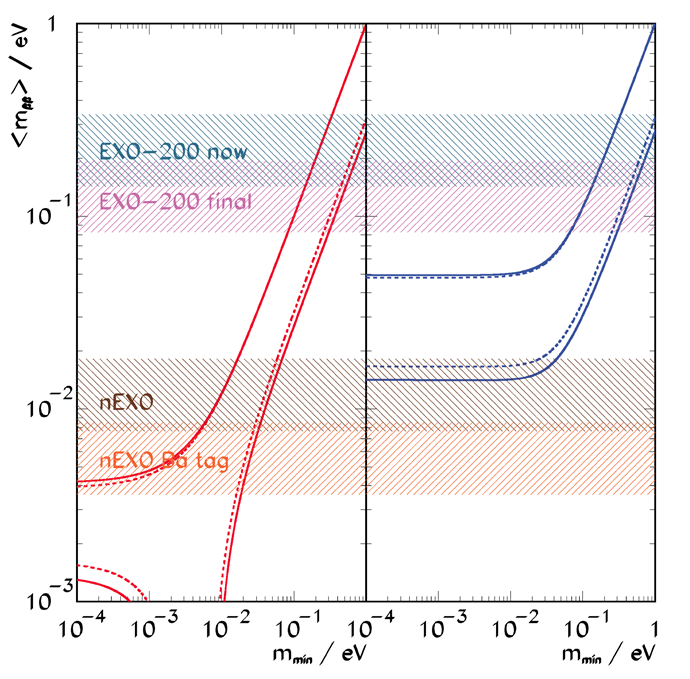
\includegraphics[width=.7\textwidth]{figures/sensitivity_v2.png}
	\caption{nEXO projected sensitivity to the Majorana neutrino mass vs. the sum of the three masses M$_{total}$. {\color{red}Is there an updated version?}}
\label{fig:sensitivity_nEXO}
\end{figure}

A schematic of the experimental setup is shown in Fig. \ref{fig:nEXO_cryopit} in one of the possible locations for nEXO, the SNOLAB cryopit.  Similar to EXO-200, the copper-housed TPC will be submerged in HFE fluid, inside a copper cryostat.  The cryostat will be insulated and submerged in a large volume of water shielding, in which photo-multiplier tubes could provide muon veto by observing Cherenkov radiation.

nEXO will be a single TPC with charge and light readouts at opposing ends of the TPC.  Rather than wires, nEXO will use tile electrodes for charge readout, shown in Fig. \ref{fig:nEXO_readout}.

\begin{figure}[H]
	\centering
	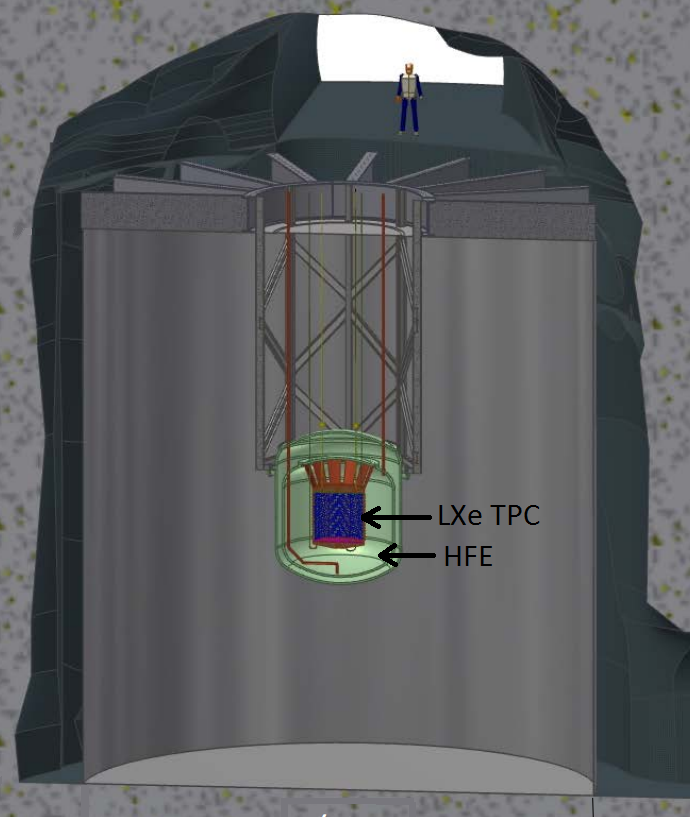
\includegraphics[width=.7\textwidth]{figures/nEXO_cryopit.png}
	\caption{nEXO in the SNOLAB cryopit. {\color{red}Needs labels}}
\label{fig:nEXO_cryopit}
\end{figure}

\begin{figure}[H]
	\centering
	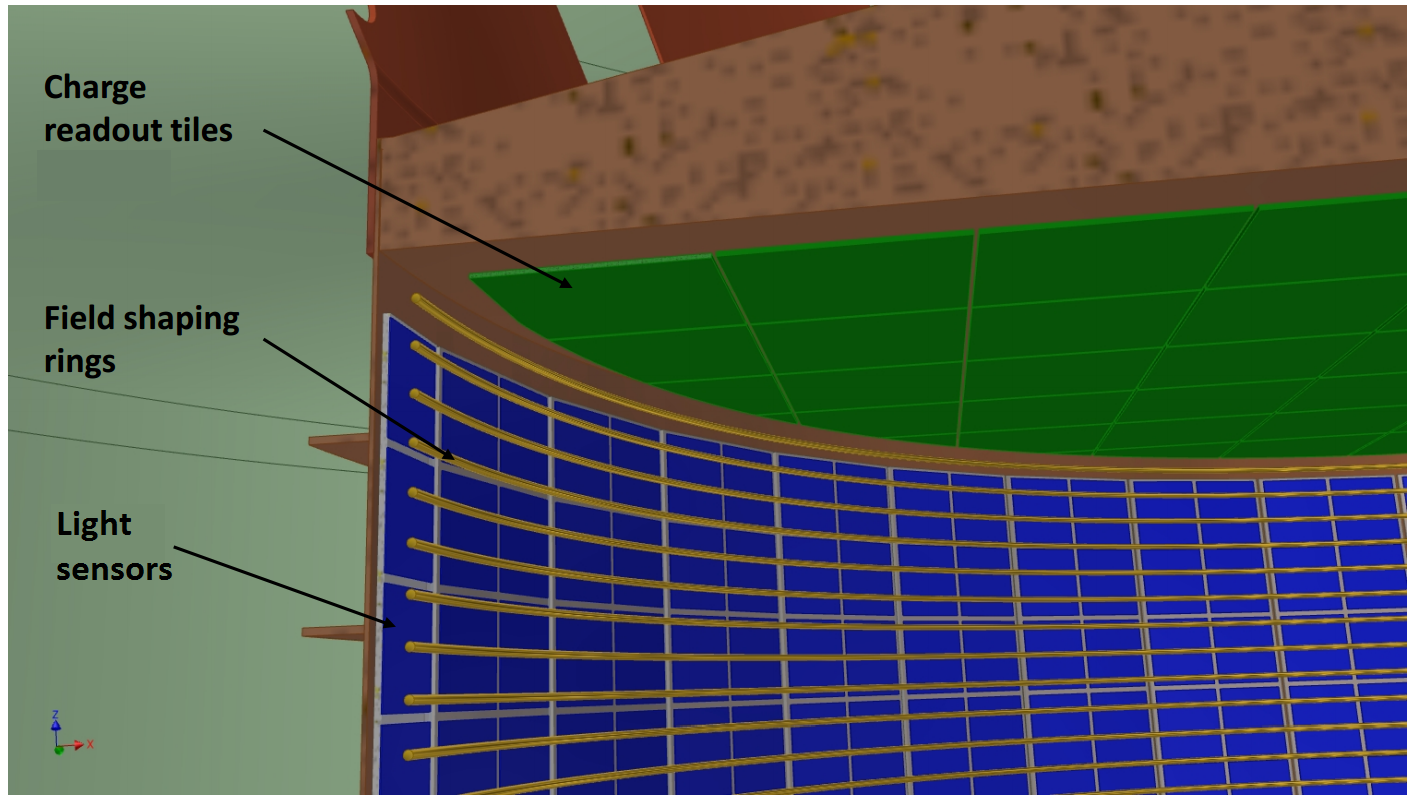
\includegraphics[width=.7\textwidth]{figures/nEXO_readout.png}
	\caption{nEXO readout.}
\label{fig:nEXO_readout}
\end{figure}

\subsection{Barium Tagging}

The backgrounds observed around the Q-value in EXO-200 can be expected to scale up with the size of nEXO.  But with the veto power of barium tagging, nEXO's sensitivity to $0\nu\beta\beta$ scales with the total \textsuperscript{136}Xe mass in the detector, vs. the square root of that mass without barium tagging [ref].

Several possible barium tagging techniques have been proposed.  Perhaps the most natural concept is to direct one or more lasers at the decay site to induce fluorescence of the barium daughter.  This technique was explored thoroughly by Fairbank's group, and was abandoned when reliable fluorescence of Ba\textsuperscript{+} in LXe could not be observed [ref Kendy's thesis].

Another concept was to grab the daughter in SXe on a cold probe, similar to the method explored in this thesis, but to then evaporate the SXe and drift the daughter into a trap for detection in vacuum.  This method was abandoned when extraction of barium from SXe samples could not be achieved by Liang Yang's group [ref?].

Two barium tagging techniques continue to be explored.  One of these is to grab the daughter on a surface, brought to the decay site by a probe, and then move it to a location where it can be desorbed from that surface by an infrared laser, and subsequently resonantly ionized by two lasers in order to detect it by time-of-flight spectroscopy {\color{red}(or other trap/detect methods?)}.  The apparatus for the study of this method is described in [instrumentation paper], along with some initial results.

The other remaining technique for barium tagging, now the concentration of Fairbank's group and the subject of this thesis, is what we call tagging in SXe.  Here, we would send a cold probe to the site of the candidate $0\nu\beta\beta$ event in order to trap the Ba/Ba\textsuperscript{+} in a small amount of SXe, and then observe it by its laser-induced fluorescence in the SXe, a technique called matrix isolation spectroscopy.

A concept for a probe is shown in Fig. [ref fig cryoprobe].  The SXe forms on a sapphire window or plug.  Sapphire is a good candidate for a substrate; it has good thermal conductivity at low temperature, is extremely transparent, and can be purified to contain low amounts of fluorescing impurities such as Cr\textsuperscript{3+}.  An excitation laser would be brought into the probe through a fiber, and aimed through the sapphire to excite the Ba/Ba\textsuperscript{+} in the SXe.  A return fiber could collect the laser reflections and used for measure the SXe thickness via interference fringes.  {\color{red}\textbf{[in the fig., label things like the fibers like (A), (B), and just say what those are in the caption]}}  The Ba/Ba\textsuperscript{+} fluorescence would then be collected by a lens/filter system and imaged onto a CCD.  Additional components, not shown, would be required for cooling the sapphire, either by liquid He or by a Joule-Thompson nozzle, as well as a thermometer.

The next chapter describes theory relevant to single Ba/Ba\textsuperscript{+} detection in SXe matrices.